\section{Geraden}
%
%
%
\subsection{Definition: (Gerade)}
%
%
%
Eine Gerade $l$ in $\mathbb{R}^{2}$ ist eine Menge der Form $l=a+\mathbb{R}b=\{a+\lambda b|\lambda \in \mathbb{R}\}$ für $b \neq (0)$\\
$a:$ "`Stützvektor"' \quad $b:$ "`Richtungsvektor"', \quad $b^{\perp}=\begin{pmatrix}-b_{2} \\ b_{1} \end{pmatrix}:$ "`Normalenvektor"'
%
\subsubsection{Beispiel: }
$a=\begin{pmatrix} 0 \\ 2 \end{pmatrix}, b=\begin{pmatrix} 3 \\ -1 \end{pmatrix}$
\begin{figure}[H]
	\centering
	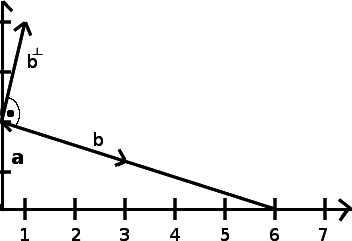
\includegraphics[width=0.3\textwidth]
	{mainmatter/chapter1/pics/orthovek.png}
	\caption{Gerade mit orthogonalen Vektor} 
\end{figure}



\subsection{Satz 1.2}
Eine Teilmenge von $\mathbb{R}^{2}$ ist eine Gerade genau dann, wenn sie Lösungsmenge einer Gleichung \\
$\{\begin{pmatrix}x \\ y \end{pmatrix} \in \mathbb{R}^{2} : \alpha x + \beta y = \gamma\}$ ist. $\alpha$ und $\beta$ nicht beide Null.
%
%
%
\subsubsection{Beweis:}
$l=a + \mathbb{R}b$\\
Dann erfüllt jeder Punkt $(a_{1}+tb_{1},a_{2}+tb_{2})$ die Gleichung $b_{2}a_{1}-b_{1}a_{2} = b_{2}x-b_{1}y$.\\
DENN:  $b_{2}(a_{1}+tb_{1})-b_{1}(a_{2}+tb_{2})=b_{2}a_{1}-b_{1}a_{2}=det(a,b)$ Erfüllt umgekehrt $\begin{pmatrix}x \\ y \end{pmatrix}$ die Gleichung $\alpha x + \beta y = \gamma$ und ist $\alpha \neq 0$, dann folgt $x=\frac{-\beta}{\alpha}y+\frac{\gamma}{\alpha}$. \\ 
Also ist $\begin{pmatrix}x \\ y \end{pmatrix}$ ein Punkt der Geraden $a + \mathbb{R}b$ mit $a=\begin{pmatrix} \frac{\gamma}{\alpha} \\ 0 \end{pmatrix}, b=\begin{pmatrix} -\beta \\ \alpha \end{pmatrix}$\\
%
%
%
\subsubsection{Beispiel:} 
\begin{equation*}
x-y=1 \qquad a=\begin{pmatrix} 1 \\ 0 \end{pmatrix} b=\begin{pmatrix} 1 \\ 1 \end{pmatrix}
\end{equation*}
\begin{figure}[H]
	\centering
	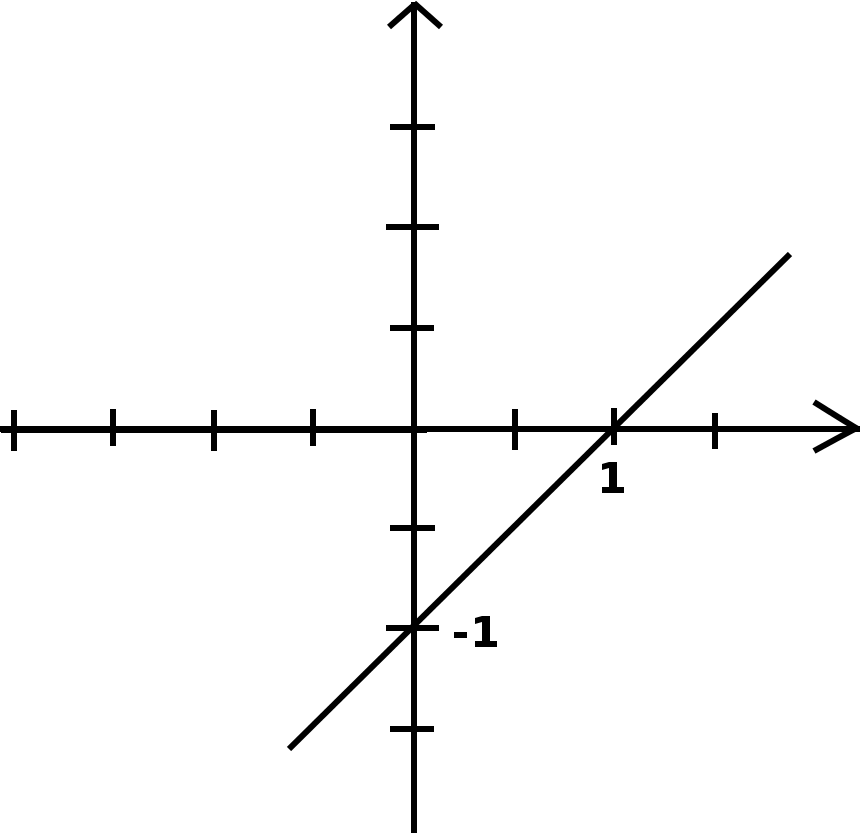
\includegraphics[width=0.3\textwidth]
	{mainmatter/chapter1/pics/bsp12.png}
	\caption{Beispiel zu Satz 1.2} 
\end{figure}